% Example LaTeX document for GP111 - note % sign indicates a comment
\documentclass{article}

\usepackage{graphicx}
\usepackage{titlesec}
\usepackage{titling}

\graphicspath{ {images/} }

\titleformat{\section}
{\normalfont\normalsize\bfseries}{\thesection}{1em}{}

\posttitle{\par\end{center}}
\setlength{\droptitle}{-20pt}

% Default margins are too wide all the way around. I reset them here
\setlength{\topmargin}{-.5in}
\setlength{\textheight}{9in}
\setlength{\oddsidemargin}{.125in}
\setlength{\textwidth}{6.25in}

\begin{document}
\title{Multi-Process Matrix Multiply using MPI \\ \large A Comparison Between Dense and Sparse Implementations}
\author{Jesse Bannon\\
University of Washington, Tacoma}
\renewcommand{\today}{July 19, 2017}
\maketitle

In this assignment, I outline the performance characteristics between a multi-process implementation of sparse and dense matrix-matrix multiply $C = AB$ using MPI. Each implementation stores matrices row-major in memory and uses double-precision floating points. These metrics were gathered on the UW 16-node virtual cluster.  Each process is ran with a single thread.

\paragraph{Dense Multiply}
The master node $p_{0}$ partitions $A$ by consecutive rows to form submatrices $A_{i}$, and sends each process $p_{i}$ both $A_{i}$ and $B$ asynchronously to compute $C_{i} = A_{i}B$. Once $C_{i}$ is computed, $p_{i}$ sends $C_{i}$ to $p_{0}$ to its respective location to form $C$.

\paragraph{Sparse Multiply}
The master node $p_{0}$ partitions the sparse elements of $A$ evenly amongst all $p_{i}$, forming $A'_{i}$. $p_0$ sends each process $p_i$ $A'_{i}$ and $B$ to compute $C'_i = A'_{i}B$. $C'_i$ is then collected by $p_{0}$ to compute $C = \sum_{i=0} C'_i$.

\begin{figure}[h]      
	\centering 
    \fbox{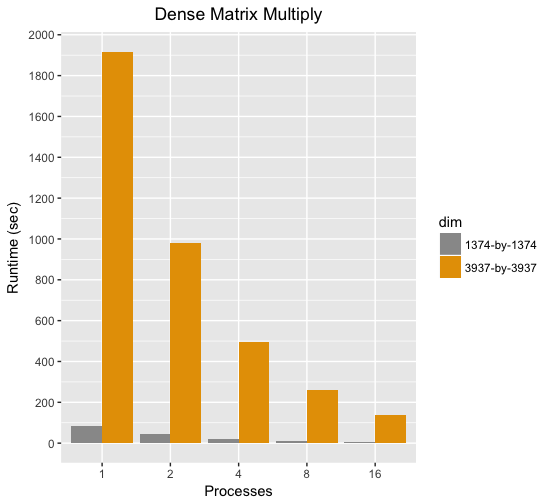
\includegraphics[width=.3\textwidth]{dense_mpi.png}}   
    \hspace{10px}
    \fbox{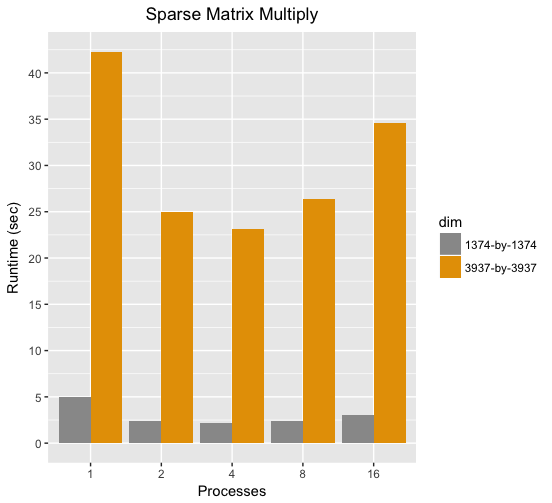
\includegraphics[width=.3\textwidth]{sparse_mpi.png}}
    \hspace{10px}
    \caption{Elapsed time to perform dense and sparse matrix-matrix multiply using MPI}
    \label{materialflowChart}
\end{figure}

The dense multiply runtime scales linearly with respect to additional processes. The sparse multiply peaks at four nodes and degrades when adding more nodes. This is most likely caused by the serialized code execuded on $p_0$ during the aggregation stage, when computing $C = \sum_{i=0} C'_i$. The better approach would be to perform a reduce when computing $C$ to take all the computional burden off $p_0$.

\paragraph{Conclusion}
The dense matrix multiply distributed the workload successfully whereas the sparse matrix multiply suffered from a bottleneck at the aggregation stage. Despite that, I learned efficient scripting techniques to manage a homogeneous cluster.

\end{document}